\documentclass[aspectratio=169]{beamer}
\usepackage{graphics,amssymb,amsfonts,amsmath}
\usepackage{pgf,tikz}
\usetikzlibrary{shapes,shapes.geometric,positioning,trees}
\DeclareGraphicsExtensions{.jpg,.pdf,.mps,.png}
\usepackage[utf8]{inputenc}
\usepackage[brazil]{babel}
\usepackage[normalem]{ulem}
\usepackage{standalone}
\usepackage{pgfpages,enumerate,hyperref}
\usepackage{palatino}   %Fonte sem serifa.
\usepackage{ragged2e}   %Par\'agrafo justificado.
\usepackage{minted}
\usepackage{tikz}
% \usetheme{CambridgeUS}
% \usetheme{AnnArbor}
% \usecolortheme{lily}
\usecolortheme{orchid}
\usefonttheme[onlymath]{serif}

\def\theFancyVerbLine{%
  \rmfamily\tiny\arabic{FancyVerbLine}%
  {\tikz[remember picture,overlay]\node(minted-\arabic{FancyVerbLine}){};}%
}

%colocando n\'umero de p\'aginas no slide.
\setbeamertemplate{footline}[frame number]

% desativando os botoes de navegacao.
\beamertemplatenavigationsymbolsempty

%Tela cheia
\hypersetup{pdfpagemode=FullScreen}

% Layout da p\'agina
\hypersetup{pdfpagelayout=SinglePage,urlcolor=blue,colorlinks=true}

% Ambiente bash
\newminted{bash}{bgcolor=gray}

% Ambiente python
\newminted{python}{bgcolor=green!25!white,linenos}

% Ambiente html
\newminted{html}{bgcolor=cyan!25,linenos}

\tikzstyle{every node}=[anchor=west]
\tikzstyle{selected}=[draw=red,fill=green!30]
\tikzstyle{optional}=[dashed,fill=gray!50]

\title{Gráficos: Django + Highcharts}
\author{R\'egis da Silva Santos\\ {\texorpdfstring{\color{blue}}{ }http://rg3915.github.io}}
\institute{\url{github.com/grupy-sp/encontros}}
\date{04 de Junho de 2016}

\begin{document}
\justifying %Par\'agrafo justificado.

%Neste caso insere somente no primeiro slide.
{%
%\usebackgroundtemplate{\centering \vspace*{5cm} \includegraphics[width=\paperwidth]{figuras/djangoPython}}

% \usebackgroundtemplate{%
% \vbox to \paperheight{\vfil\hbox to \paperwidth{\hfil\includegraphics[width=\paperwidth]{img/logo_mascote.jpg}\hfil}\vfil}
% }

% \begin{frame}

% \end{frame}
% }

\begin{frame}
	\titlepage
\end{frame}

\begin{frame}\frametitle{Django}
Se você não conhece Django sugiro que leia este tutorial.

\

\url{http://pythonclub.com.br/tutorial-django-17.html}

\

Além da documentação oficial.

\

\url{https://docs.djangoproject.com/en/1.9/intro/tutorial01/}

\

\begin{center}
    \large Django==1.9.6
\end{center}
\end{frame}

\begin{frame}\frametitle{Highcharts}

    \begin{center}
        \url{http://www.highcharts.com/}
    \end{center}

    \begin{figure}[h]
      \centering
        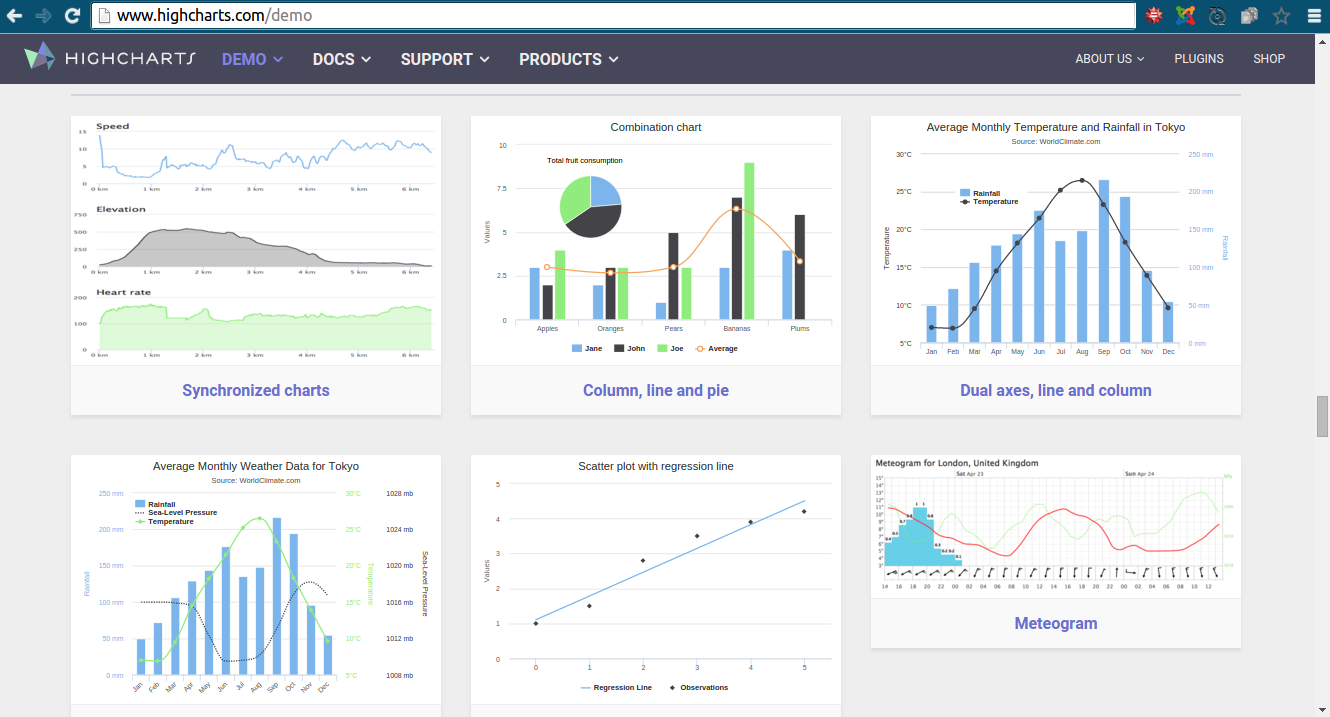
\includegraphics[width=.8\paperwidth]{img/demo.png}
    \end{figure}

\end{frame}

\begin{frame}\frametitle{Objetivo}

    \begin{figure}[h]
      \centering
        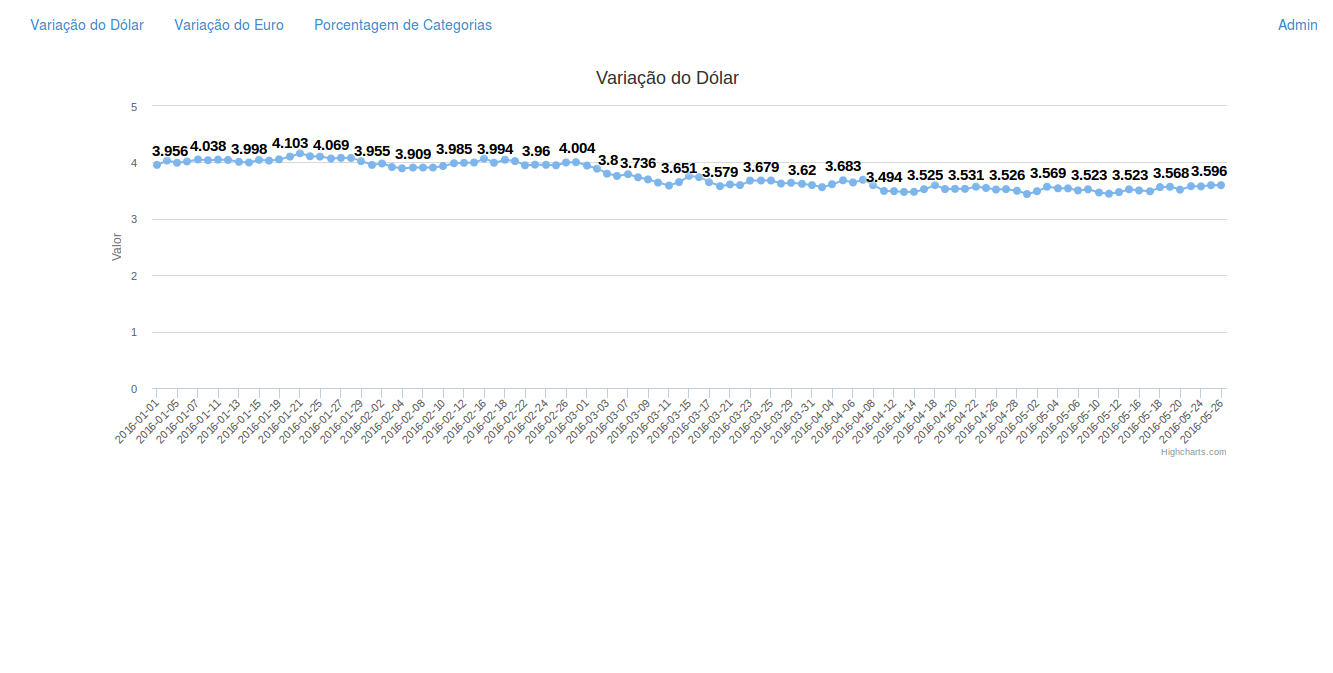
\includegraphics[width=.9\paperwidth]{img/dollar.png}
    \end{figure}

\end{frame}

\begin{frame}[fragile]\frametitle{Começando...}

\begin{bashcode}
$ git clone https://github.com/rg3915/highcharts.git
$ cd highcharts
$ source setup.sh
\end{bashcode}

\end{frame}

\begin{frame}[fragile]\frametitle{Modelo}

\begin{pythoncode}
# models.py
from django.db import models


class Dollar(models.Model):
    date = models.DateField('data')
    value = models.DecimalField('valor', max_digits=4,
                                decimal_places=3)


class Euro(models.Model):
    date = models.DateField('data')
    value = models.DecimalField('valor', max_digits=4,
                                decimal_places=3)
\end{pythoncode}

\end{frame}

\begin{frame}[fragile]\frametitle{}

\begin{pythoncode}
class Category(models.Model):
    category = models.CharField('categoria', max_length=50,
                                unique=True)


class Product(models.Model):
    category = models.ForeignKey('Category',
                                 verbose_name='categoria')
    product = models.CharField('Produto', max_length=60,
                               unique=True)
    price = models.DecimalField('Preço', max_digits=6,
                                decimal_places=2)
\end{pythoncode}

\end{frame}

\begin{frame}[fragile]\frametitle{Importando os dados de um CSV}

Variação do dólar

\url{http://www.dolarhoje.net.br/dolar-comercial.php}

\

\begin{pythoncode}
# dollar.csv
date,value
1/1/2016,3.956
4/1/2016,4.033
5/1/2016,3.994
6/1/2016,4.017
7/1/2016,4.052
8/1/2016,4.038
11/1/2016,4.049
...
\end{pythoncode}

\

Variação do euro

\url{http://br.investing.com/currencies/eur-brl-historical-data}

\end{frame}

\begin{frame}[fragile]\frametitle{}

\begin{pythoncode}
# shell_dollar.py
import csv
import datetime as dt
from highcharts.core.models import Dollar

dollar_list = []
with open('highcharts/fix/dollar.csv', 'r') as f:
    r = csv.DictReader(f)
    for dct in r:
        # Convert '%d/%m/%Y' to '%Y-%m-%d'.
        d = dt.datetime.strptime(dct['date'], '%d/%m/%Y')\
                       .strftime('%Y-%m-%d')
        dollar_list.append((d, dct['value']))
    f.close()

obj = [Dollar(date=val[0], value=val[1]) for val in dollar_list]
Dollar.objects.bulk_create(obj)
\end{pythoncode}

\end{frame}

\begin{frame}[fragile]\frametitle{Importando os dados via shell}

\begin{bashcode}
python manage.py shell < highcharts/shell/shell_dollar.py
\end{bashcode}

\end{frame}

\begin{frame}[fragile]\frametitle{graphics.py}

\begin{pythoncode}
# graphics.py
import json
from django.db.models import Count
from django.core.serializers.json import DjangoJSONEncoder
from django.http import HttpResponse
from .models import Dollar, Euro, Product


def dollar_json(request):
    data = Dollar.objects.values('date', 'value')
    lista = [{'dia': i['date'], 
              'valor': float(i['value'])} for i in data]
    resp = json.dumps(lista, cls=DjangoJSONEncoder)
    return HttpResponse(resp)
\end{pythoncode}

\end{frame}

\begin{frame}[fragile]\frametitle{graphics.py}

\begin{pythoncode}
def euro_json(request):
    data = Euro.objects.values('date', 'value')
    lista = [{'dia': i['date'], 
              'valor': float(i['value'])} for i in data]
    resp = json.dumps(lista, cls=DjangoJSONEncoder)
    return HttpResponse(resp)
\end{pythoncode}

\end{frame}

\begin{frame}[fragile]\frametitle{urls.py}

\begin{pythoncode}
# urls.py
from django.conf.urls import include, url
from django.contrib import admin

urlpatterns = [
    url(r'', include('highcharts.core.urls', namespace='core')),
    url(r'^admin/', include(admin.site.urls)),
]
\end{pythoncode}

\end{frame}

\begin{frame}[fragile]\frametitle{core/urls.py}

\begin{pythoncode}
# core/urls.py
from django.conf.urls import url
from highcharts.core.graphics import dollar_json, euro_json, product_json
from highcharts.core import views as v

urlpatterns = [
    url(r'^$', v.home, name='home'),
    url(r'^dollar-graphic/$', v.dollar_graphic, name='dollar-graphic'),
    url(r'^euro-graphic/$', v.euro_graphic, name='euro-graphic'),
    url(r'^product-graphic/$', v.product_graphic, name='product-graphic'),
    url(r'^dollar_json/$', dollar_json),
    url(r'^euro_json/$', euro_json),
    url(r'^product_json/$', product_json),
]
\end{pythoncode}

\end{frame}

\begin{frame}[fragile]\frametitle{Views}
    
\begin{pythoncode}
# views.py
from django.shortcuts import render

def home(request):
    return render(request, 'index.html')

def dollar_graphic(request):
    return render(request, 'dollar_graphic.html')

def euro_graphic(request):
    return render(request, 'euro_graphic.html')

def product_graphic(request):
    return render(request, 'product_graphic.html')
\end{pythoncode}

\end{frame}

\begin{frame}[fragile]\frametitle{Templates}

Dentro da pasta \texttt{highcharts/core/} crie a pasta \texttt{templates}.

\

\begin{bashcode}
mkdir templates
touch templates/base.html
touch templates/dollar_graphic.html
touch templates/euro_graphic.html
touch templates/product_graphic.html
\end{bashcode}

\end{frame}

\begin{frame}[fragile]\frametitle{base.html}
    
\begin{htmlcode}
# base.html

<html>
<head>
  <!-- jQuery -->
  <script src=""></script>
  <!-- HighCharts JS -->
  <script src=""></script>
</head>
<body>
  
  <div class="container">
    
    
  </div>
</body>
</html>
\end{htmlcode}

\end{frame}

\begin{frame}[fragile]\frametitle{dollar\_graphic.html}

\begin{htmlcode}
# dollar_graphic.html




  <div id="dollar-chart"></div>



  <script src=""></script>

\end{htmlcode}

\end{frame}

\begin{frame}[fragile]\frametitle{}

Crie a pasta \texttt{static/js}.

\

\begin{bashcode}
mkdir -p static/js
touch static/js/dollar_graphic.js
touch static/js/euro_graphic.js
touch static/js/product_graphic.js
\end{bashcode}

\end{frame}

\begin{frame}[fragile]\frametitle{dollar\_graphic.js}

\begin{htmlcode}
# dollar_graphic.js
$(function () {
    var url = "/dollar_json/";

    $.getJSON(url, function(res){
        /* Transformando o dicionário em lista.
           Com o comando map eu coloco uma lista dentro da outra,
           necessário para este tipo de gráfico. */
        var data = res.map(function (v) {
            return [v.dia, v.valor]
        });
\end{htmlcode}

\end{frame}

\begin{frame}[fragile]\frametitle{dollar\_graphic.js}

\begin{htmlcode}
        $('#dollar-chart').highcharts({
            chart: {
                type: 'line'
            },
            title: {
                text: 'Variação do Dólar'
            },
            xAxis: {
                type: 'category'
            },
\end{htmlcode}

\end{frame}

\begin{frame}[fragile]\frametitle{dollar\_graphic.js}

\begin{htmlcode}
            yAxis: {
                min: 0,
                title: {
                    text: 'Valor'
                },
                plotOptions: {
                    line: {
                        dataLabels: {
                            enabled: true
                        },
                    }
                },
            },
            legend: {
                enabled: false
            },
\end{htmlcode}

\end{frame}

\begin{frame}[fragile]\frametitle{dollar\_graphic.js}

\begin{htmlcode}
            series: [{
                data: data,
                dataLabels: {
                    enabled: true,
                    align: 'center',
                    style: {
                        fontSize: '15px'
                    }
                }
            }],
        });
    });
});
\end{htmlcode}

\end{frame}

\begin{frame}

    \begin{figure}[h]
      \centering
        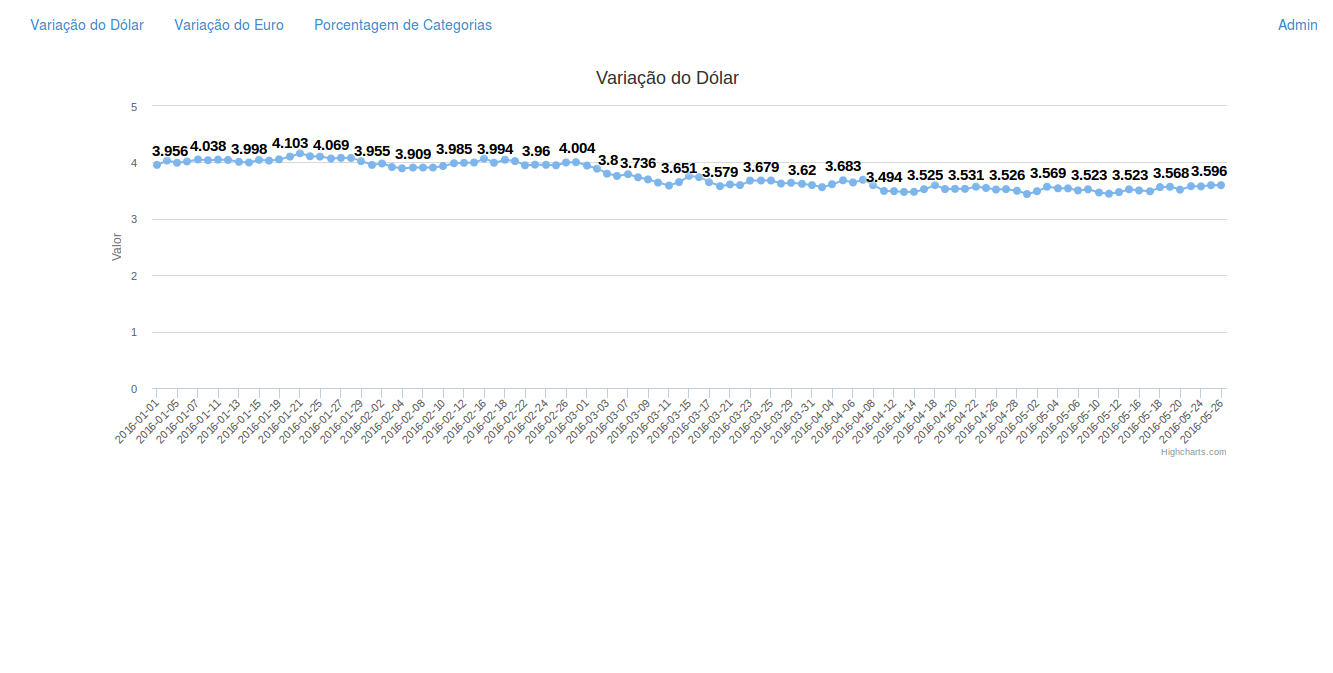
\includegraphics[width=\paperwidth]{img/dollar.png}
    \end{figure}

\end{frame}

\begin{frame}

    \begin{figure}[h]
      \centering
        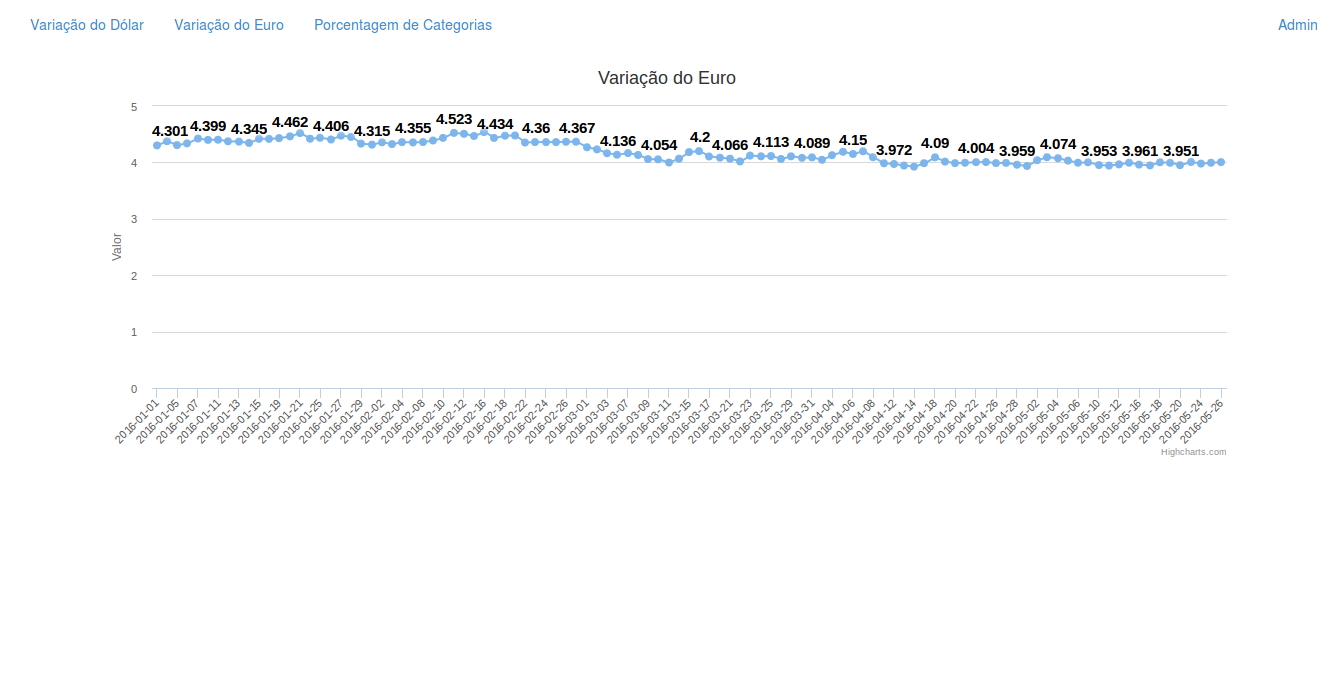
\includegraphics[width=\paperwidth]{img/euro.png}
    \end{figure}

\end{frame}

\begin{frame}[fragile]\frametitle{graphics.py}

\begin{pythoncode}
def product_json(request):
    ''' Porcentagem de produtos por categoria '''
    data = Product.objects.values('category')\
        .annotate(value=Count('category'))\
        .order_by('category')\
        .values('category', 'category__category', 'value')
    total = Product.objects.all().count()
    '''Podemos reescrever o dicionário com nossos próprios 
    nomes de campos. '''
    lista = [{'categoria': item['category__category'],
        'porcentagem': float((item['value'] / total) * 100)} 
        for item in data]
    s = json.dumps(lista, cls=DjangoJSONEncoder)
    return HttpResponse(s)
\end{pythoncode}


\end{frame}

\begin{frame}[fragile]\frametitle{product\_graphic.js}

\begin{htmlcode}
$(function () {
    var url = "/product_json/";

    $.getJSON(url, function(res){
        /* Transformando o dicionário em lista.
           Com o comando map eu coloco uma lista dentro da outra,
           necessário para este tipo de gráfico. */
        var data = res.map(function (v) {
            return [v.categoria, v.porcentagem]
        });
\end{htmlcode}

\end{frame}


\begin{frame}[fragile]\frametitle{product\_graphic.js}

\begin{htmlcode}
        $('#product-chart').highcharts({
            chart: {
                type: 'pie'
            },
            title: {
                text: 'Porcentagem de produtos por categoria'
            },
            tooltip: {
                pointFormat: '<b>{point.percentage:.1f}%</b>'
            },
            plotOptions: {
                pie: {
                    allowPointSelect: true,
                    cursor: 'pointer',
                    dataLabels: {
                        enabled: true,
                        format: '<b>{point.name}</b>: {point.percentage:.1f} %'
                    }
                }
            },
\end{htmlcode}

\end{frame}


\begin{frame}[fragile]\frametitle{product\_graphic.js}

\begin{htmlcode}
            series: [{
                name: 'Categoria',
                colorByPoint: true,
                data: data
            }],
        });
    });
});
\end{htmlcode}

\end{frame}



\begin{frame}

    \begin{figure}[h]
      \centering
        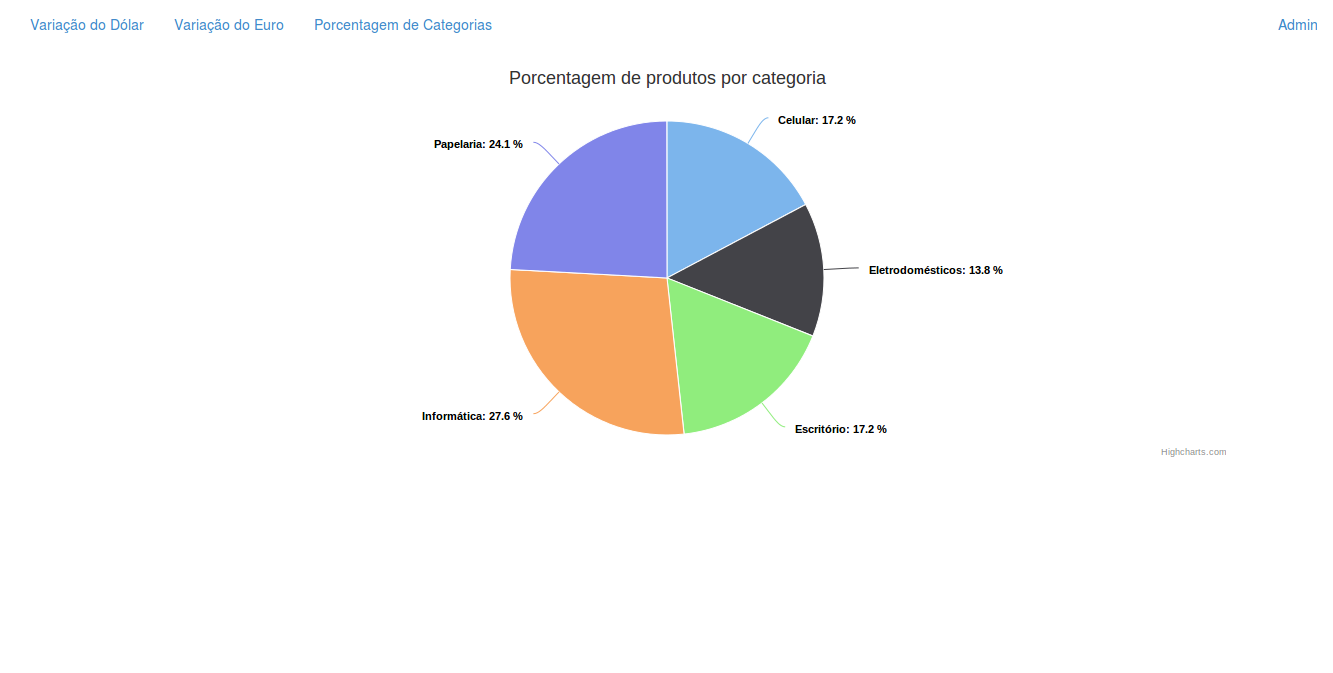
\includegraphics[width=\paperwidth]{img/product.png}
    \end{figure}

\end{frame}

\begin{frame}
	\centering
	\huge Obrigado!

	\

	\

	\large Dúvidas?
\end{frame}

\begin{frame}
	\titlepage
\end{frame}

\end{document}